\subsection{Hazard Unit}

The test bench for the hazard unit ensures that the stall and flush signal is asserted when the input is as described in section \ref{sec:hazard_unit}. A screenshot of the test bench executed in Modelsim is included the attachments.


\subsection{Branch Prediction}

The branch prediction test bench verifies that the branch prediction unit uses it internal table to store and predict branches. Figure \ref{fig:branch_prediction_tb} shows what happens to the prediction table if a branch which is in state TAKEN\_STRONG and the branch address is not taken three times in a row.

\begin{figure}[h]
        \centerline{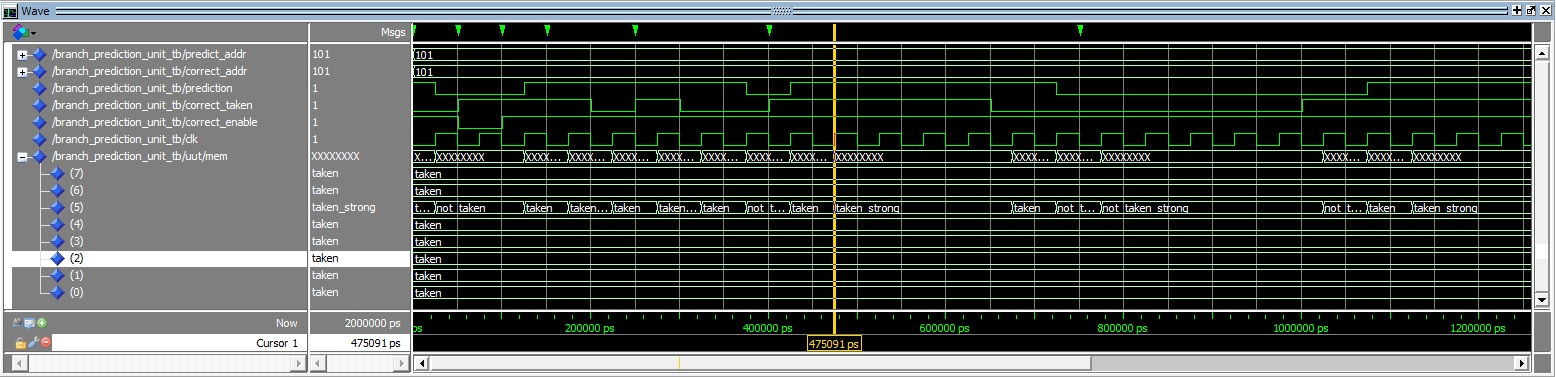
\includegraphics[width=600px]{figures/tb/branch_prediction.jpg}}
        \caption{The branch\_prediction test bench}
        \label{fig:branch_prediction_tb}
\end{figure}
\FloatBarrier

Here the branch address is constanlty 5 and the branch is simulated to repeatedly be not taken, by deasserting the \emph{correct\_taken} signal for four consecutive cycles. From the yellow marker the memory location 5 in the branch unit takes the states TAKEN\_STRONG, TAKEN, NOT\_TAKEN and NOT\_TAKEN\_STRONG. This proves that the branch prediction unit updates it table correctly. By observing the prediction made in the same time period which is high for the states TAKEN\_STRONG and TAKEN and transitions to low when the state changes to NOT\_TAKEN and stays there for the NOT\_TAKEN\_STRONG state.

\subsection{Forwarding Unit} 

This unit checks the registers used in the memory, execute, instruction decode and write back stages and asserts the four forwarding signals A, B, C, D. In the test bench different combinations of the registers are set up and the outputs are asserted. A screenshot of the execution is attached.